\chapter{Arhitektura i dizajn sustava}		
	
	Sustav se može podijeliti na podsustave:
		\begin{packed_item}
			
			\item  Klijent
			\item  Poslužitelj
			\item  Baza podataka
			
		\end{packed_item}
	
		\begin{figure}[H]
			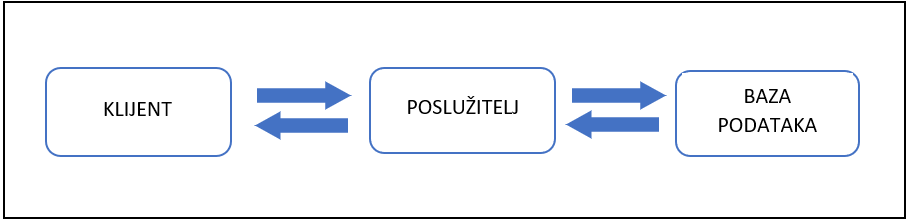
\includegraphics[width=\textwidth]{slike/Organizacija_sustava.PNG} %veličina u odnosu na širinu linije
			\caption{Organizacija sustava}
			\label{fig:organizacija_sustava1} %label mora biti drugaciji za svaku sliku
		\end{figure}
		
 
\underbar{Klijent} je web preglednik pomoću kojeg korisnici pristupaju našoj web aplikaciji. Često korišteni web preglednici su: Google Chrome, Apple Safari, Mozilla Firefox. Kada korisnik pristupa web aplikaciji, web preglednik šalje HTTP (\textit{engl. Hypertext Transfer Protocol}) zahtjeve za preuzimanje statičkih datoteka web poslužitelju. Statičke datoteke mogu biti HTML, CSS i JavaScript (React.js) datoteke. Nakon preuzimanja datoteka, preglednik ih koristi za izgradnju i prikaz korisničkog sučelja te izvršavanje funkcija unutar aplikacije. 

\underbar{Poslužitelj} je Python aplikacija pisana unutar web mikrookvira Flask. On služi kao posrednik između  klijenta (korisničkog sučelja) i baze podataka. U Python aplikaciji (Flask aplikaciji) definirani su RESTful API-ji (kao rute ili krajnje točke) koji omogućuju klijentima da šalju HTTP zahtjeve za određenim podacima. Prilikom obrade tih zahtjeva, Python aplikacija šalje upite bazi podataka kako bi dohvatila, promijenila ili dodala željene podatke.

Kada \underbar{baza podataka} zaprimi upite od poslužitelja, ona ih izvršava i vraća rezultate poslužitelju. Vraćeni rezultati mogu biti u obliku potvrde o izvršenom upitu ili u obliku podataka koje je poslužitelj zatražio od baze podataka. Baza podataka ostaje pasivna sve dok ne zaprimi nove upite od poslužitelja.

Aplikacija je organizirana po MVC (\textit{engl. Model-View-Controller, hrv. Model-Pogled-Nadglednik}) obrascu.  

Općenito, \textit{Model} definira podatke, njihovu strukturu i operacije koje se mogu izvršavati nad tim podacima. \textit{Pogled} predstavlja prikaz podataka korisniku (npr. korisničko sučelje).
\textit{Nadglednik} predstavlja posrednike između Modela i Pogleda. Oni obrađuju zahtjeve korisnika, vrše operacije nad Modelom i ažuriraju Pogled. Organizacija po ovom obrascu olakšava proširivanje i održavanje aplikacije.

Naša aplikacija ne sadrži doslovno sve tri navedene komponente. Ovdje Python objedinjuje Model i dio logike Nadglednika. Komponente u React-u odgovaraju Pogledu te je i ovdje sadržan dio logike Nadglednika.

				
		\section{Baza podataka}

Za rješavanje projektnog zadatka odabrana je relacijska baza podataka. Implementirali smo je korištenjem sustava PostgreSQL. To je besplatan sustav za upravljanje bazom podataka otvorenog koda. Objekti relacijske baze podataka su relacije. Neformalno, i u PostgreSQL-u, to su dvodimenzionalne imenovane tablice gdje imenovani stupac predstavlja atribut, a redak zapis relacije. Izbor ovakve baze podataka omogućio nam je lakše strukturiranje podatka i definiranje veza između njih, normalizaciju, skalabilnost te sigurnost kod pohrane i dohvata podataka. 
Zbog potreba naše aplikacije, baza podataka sadrži entitete:

        \begin{packed_item}
		\item 	\textnormal{Korisnik}
		\item 	\textnormal{Djelatnik}
        \item 	\textnormal{Pacijent}
        \item 	\textnormal{Terapija}
        \item 	\textnormal{VrstaTerapije}	
        \item 	\textnormal{Termin}			
        \item 	\textnormal{Status}		
        \item 	\textnormal{Soba}	
        \item 	\textnormal{Uredaj}
        \item 	\textnormal{VrstaUredaja}
        \item    SobaZa
                   				
	 \end{packed_item}

		
			\subsection{Opis tablica}
			
\textbf{Korisnik:}

Entitet Korisnik sadrži sve bitne informacije o korisniku aplikacije. Entitet sadrži atribute: idKorisnika, ime, prezime, datumRodenja, telefon, email, lozinka. Atribut idKorisnika je primarni ključ. Atributi email i telefon su alternativni ključevi. Korisnik može biti ili djelatnik zdravstvene ustanove ili pacijent koji se želi naručiti na terapiju u zdravstvenoj ustanovi. 

				
				
				\begin{longtblr}[
					label=none,
					entry=none
					]{
						width = \textwidth,
						colspec={|X[6,l]|X[7, l]|X[20, l]|}, 
						rowhead = 1,
					} %definicija širine tablice, širine stupaca, poravnanje i broja redaka naslova tablice
					\hline \SetCell[c=3]{c}{\textbf{Korisnik}}	 \\ \hline[3pt]
					\SetCell{LightGreen}idKorisnika & INT & jedinstveni identifikator korisnika 	\\ \hline
					ime & VARCHAR(50) & ime korisnika	\\ \hline 
                     prezime & VARCHAR(50) & prezime korisnika	\\ \hline
                     datumRodenja & DATE & datum rođenja korisnika	\\ \hline  
                     telefon & VARCHAR(50) & broj mobilnog telefona korisnika	\\ \hline 
					email & VARCHAR(100) & e-mail adresa korisnika   \\ \hline 
					lozinka & VARCHAR(100) & hash lozinke za prijavu u aplikaciju	\\ \hline 
					 
				\end{longtblr}

\textbf{Djelatnik:}

Entitet Djelatnik je ekskluzivna specijalizacija entiteta Korisnik. Entitet sadrži atribute: idKorisnika, jeAktivan, jeAdmin, OIB. Djelatnik je povezan s Korisnikom preko atributa idKorisnika. Atribut OIB je alternativni ključ.

				\begin{longtblr}[
					label=none,
					entry=none
					]{
						width = \textwidth,
						colspec={|X[6,l]|X[7, l]|X[20, l]|}, 
						rowhead = 1,
					} %definicija širine tablice, širine stupaca, poravnanje i broja redaka naslova tablice
					\hline \SetCell[c=3]{c}{\textbf{Djelatnik}}	 \\ \hline[3pt]
					\SetCell{LightBlue}idKorisnika & INT & jedinstveni identifikator korisnika (korisnik.idKorisnika) 	\\ \hline
					OIB & CHAR(11) & osobni identifikacijski broj pacijenta	\\ \hline
					jeAktivan & BOOLEAN & označava radni odnos liječnika i zdravstvene ustanove (radi = true, ne radi = false)	\\ \hline 
					jeAdmin & BOOLEAN & označava je li djelatnik administrator (true = je, false = nije)	\\ \hline
					
					 
				\end{longtblr}

\textbf{Pacijent:}

Entitet Pacijent je ekskluzivna specijalizacija entiteta Korisnik. Entitet sadrži atribute: idKorisnika, MBO. Pacijent je povezan s Korisnikom preko atributa idKorisnika (korisnik.idKorisika). Atribut MBO je alternativni ključ.

				\begin{longtblr}[
					label=none,
					entry=none
					]{
						width = \textwidth,
						colspec={|X[6,l]|X[7, l]|X[20, l]|}, 
						rowhead = 1,
					} %definicija širine tablice, širine stupaca, poravnanje i broja redaka naslova tablice
					\hline \SetCell[c=3]{c}{\textbf{Pacijent}}	 \\ \hline[3pt]
					\SetCell{LightBlue}idKorisnika & INT & jedinstveni identifikator korisnika (korisnik.idKorisnika)	\\ \hline
					MBO & CHAR(9) & matični broj osiguranika (pacijenta)	\\ \hline 

					 
				\end{longtblr}

\textbf{Terapija:}

Entitet Terapija sadrži sve bitne informacije o terapiji na koju je pacijent naručen. Entitet sadrži atribute: idTerapije, idLijecnika, opisOboljenja, zahtPostLijec, datumPoc, datumZavrs, idPacijenta, idVrste. Atributi zahtPostLijec, datumPoc, datumZavrs i idVrste su opcionalni. Entitet Terapija je povezan binarnom N:1 vezom s entitetom Pacijentom preko atributa idPacijenta. Entitet Terapija je povezan binarnom N:1 vezom s entitetom VrstaTerapije preko atributa idVrste.

				\begin{longtblr}[
					label=none,
					entry=none
					]{
						width = \textwidth,
						colspec={|X[6,l]|X[7, l]|X[20, l]|}, 
						rowhead = 1,
					} %definicija širine tablice, širine stupaca, poravnanje i broja redaka naslova tablice
					\hline \SetCell[c=3]{c}{\textbf{Terapija}}	 \\ \hline[3pt]
					\SetCell{LightGreen}idTerapije & INT & jedinstveni identifikator terapije	\\ \hline
					idLijecnika & INT & jedinstveni identifikator liječnika	\\ \hline 
                    opisOboljenja & VARCHAR(300) & opis oboljenja pacijenta	\\ \hline
                    zahtPostLijec & VARCHAR(300) & zahtjev za postupkom liječenja (terapijom)	\\ \hline  
                    datumPoc & DATETIME & datum početka terapije	\\ \hline 
					 datumZavrs & DATETIME & datum završetka terapije   \\ \hline 
					 \SetCell{LightBlue}idPacijenta & INT & jedinstveni identifikator pacijenta (pacijent.idKorisnika)	\\ \hline 
					 \SetCell{LightBlue}idVrste & INT & jedinstveni identifikator vrste uređaja (vrstaTerapije.idVrste) \\ \hline
					 
				\end{longtblr}

\textbf{VrstaTerapije:}

Entitet VrstaTerapije sadrži sve bitne informacije o vrsti terapije na koju je pacijent naručen. Entitet sadrži atribute: idVrste, imeVrste, opisVrste. Atribut idVrste je primarni ključ. Atribut opisVrste je opcionalan. Entitet VrstaTerapije povezan je binarnom N:N vezom s entitetom Soba.

\begin{longtblr}[
					label=none,
					entry=none
					]{
						width = \textwidth,
						colspec={|X[6,l]|X[7, l]|X[20, l]|}, 
						rowhead = 1,
					} %definicija širine tablice, širine stupaca, poravnanje i broja redaka naslova tablice
					\hline \SetCell[c=3]{c}{\textbf{VrstaTerapije}}	 \\ \hline[3pt]
					\SetCell{LightGreen}idVrste & INT & jedinstveni identifikator vrste terapije	\\ \hline
					imeVrste & VARCHAR(50) & naziv vrste terapije	\\ \hline 
                     opisVrste & VARCHAR(300) & opis vrste terapije	\\ \hline
					 
				\end{longtblr}

\textbf{Termin:}

Entitet Termin sadrži sve bitne informacije o terminu terapije na koji je pacijent naručen. Entitet Termin ne postoji bez entiteta vlasnika, entiteta Terapija (Termin je egzistencijalno slab entitet). Atribut idTermina je primarni ključ, dok su idTerapije, brSobe, idStatus i idDjelatnika strani ključevi. Atributi do, komentar i idDjelatnika su opcionalni. Entitet Termin povezan je binarnom N:1 vezom s entitetom Terapija preko atributa idTerapije. Entitet Termin povezan je binarnom N:1 vezom s entitetom Soba preko atributa brSobe. Entitet Termin povezan je binarnom N:1 vezom s entitetom Status preko atributa idStatus. Entitet Termin povezan je binarnom N:0..1 vezom s entitetom Djelatnik preko atributa idKorisnika.
\textit{Napomena: Primarni ključ entiteta Termin je kompozitni ključ (idTermina, idTerapije).}

\begin{longtblr}[
					label=none,
					entry=none
					]{
						width = \textwidth,
						colspec={|X[6,l]|X[7, l]|X[20, l]|}, 
						rowhead = 1,
					} %definicija širine tablice, širine stupaca, poravnanje i broja redaka naslova tablice
					\hline \SetCell[c=3]{c}{\textbf{Termin}}	 \\ \hline[3pt]
					\SetCell{LightGreen}idTermina & INT & jedinstveni identifikator termina terapije \\ \hline
					\SetCell{LightBlue}idTerapije & INT & jedinstveni identifikator terapije (terapija.idTerapije)	\\ \hline 
					\SetCell{LightBlue}idDjelatnika & INT & jedinstveni identifikator djelatnika (djelatnik.idKorisnika)	\\ \hline
                     od & TIMESTAMP & datum i vrijeme početka termina	\\ \hline
					 do & TIMESTAMP & datum i vrijeme završetka termina      \\ \hline
                     komentar & VARCHAR(300) & komentar liječnika o napretku terapije \\ \hline
                     \SetCell{LightBlue}brSobe & VARCHAR(10) & jedinstveni identifikator sobe (soba.brSobe)	\\ \hline
                     \SetCell{LightBlue}idStatus & INT & jedinstveni identifikator statusa (status.idStatus)	\\ \hline
                                          
				\end{longtblr}

\textbf{Soba:}

Entitet Soba sadrži sve bitne informacije o sobi u kojoj se provodi neka terapija. Entitet sadrži atribute: brSobe, kapacitet, uUporabi. Atribut brSobe je primarni ključ. Entitet Soba povezan je binarnom N:N vezom s entitetom VrstaTerapije.

\begin{longtblr}[
					label=none,
					entry=none
					]{
						width = \textwidth,
						colspec={|X[6,l]|X[7, l]|X[20, l]|}, 
						rowhead = 1,
					} %definicija širine tablice, širine stupaca, poravnanje i broja redaka naslova tablice
					\hline \SetCell[c=3]{c}{\textbf{Soba}}	 \\ \hline[3pt]
					\SetCell{LightGreen}brSobe & VARCHAR(10) & jedinstveni identifikator sobe \\ \hline
                     kapacitet & INT & kapacitet sobe, broj pacijenata koji istovremeno mogu biti na terapiji u nekoj sobi	\\ \hline
                     uUporabi & BOOLEAN & označava je li soba popunjena (true = popunjena, false = nije popunjena)	\\ \hline
				\end{longtblr}
				
\textbf{SobaZa:}

Entitet SobaZa sadrži sve bitne informacije o sobi u kojoj se odvija točno određena vrsta terapije. Entitet SobaZa sadrži atribute brSobe i idVrste. Atributi brSobe i idVrste su strani ključevi. 

				\begin{longtblr}[
					label=none,
					entry=none
					]{
						width = \textwidth,
						colspec={|X[6,l]|X[7, l]|X[20, l]|}, 
						rowhead = 1,
					} %definicija širine tablice, širine stupaca, poravnanje i broja redaka naslova tablice
					\hline \SetCell[c=3]{c}{\textbf{SobaZa}}	 \\ \hline[3pt]
					\SetCell{LightBlue}brSobe & INT & jedinstveni identifikator sobe (soba.brSobe)	\\ \hline
					\SetCell{LightBlue}idVrste & INT & jedinstveni identifikator vrste terapije (vrstaTerapije.idVrste)	\\ \hline 

					 
				\end{longtblr}

\textbf{Uredaj:}

Entitet Uredaj sadrži sve bitne informacije o uređaju. Entitet sadrži atribute: idUredaja, brSobe, idVrste. Atribut idUredaja je primarni ključ, dok su atributi brSobe i idVrste strani ključevi. Atribut brSobe je opcionalan. Entitet Uredaj povezan je binarnom N:0..1 vezom s entitetom Soba preko atributa brSobe. Entitet Uredaj povezan je binarnom N:1 vezom s entitetom VrstaUredaja preko atributa idVrste.

\begin{longtblr}[
					label=none,
					entry=none
					]{
						width = \textwidth,
						colspec={|X[6,l]|X[7, l]|X[20, l]|}, 
						rowhead = 1,
					} %definicija širine tablice, širine stupaca, poravnanje i broja redaka naslova tablice
					\hline \SetCell[c=3]{c}{\textbf{Uredaj}}	 \\ \hline[3pt]
					\SetCell{LightGreen}idUredaja & INT & jedinstveni identifikator uređaja \\ \hline
                    \SetCell{LightBlue}brSobe & VARCHAR(10) & jedinstveni identifikator sobe (soba.brSobe) \\ \hline
                     \SetCell{LightBlue}idVrste & INT & jedinstveni identifikator vrste uređaja (vrstaUredaja.idVrste)\\ \hline
				\end{longtblr}

\textbf{VrstaUredaja:}

Entitet VrstaUredaja sadrži sve bitne informacije o vrsti uređaja. Entitet sadrži atribute: idVrste, imeVrste, opisVrste. Atribut idVrste je primarni ključ. Atribut opisVrste je opcionalan.

\begin{longtblr}[
					label=none,
					entry=none
					]{
						width = \textwidth,
						colspec={|X[6,l]|X[7, l]|X[20, l]|}, 
						rowhead = 1,
					} %definicija širine tablice, širine stupaca, poravnanje i broja redaka naslova tablice
					\hline \SetCell[c=3]{c}{\textbf{VrstaUredaja}}	 \\ \hline[3pt]
					\SetCell{LightGreen}idVrste & INT & jedinstveni identifikator vrste uređaja \\ \hline
                     imeVrste & VARCHAR(50) & naziv vrste uređaja \\ \hline
                     opisVrste & VARCHAR(300) & opis vrste uređaja \\ \hline
				\end{longtblr}


\textbf{Status:}

Entitet Status sadrži sve bitne informacije o statusu termina terapije koji je dodijeljen pacijentu. Entitet sadrži atribute: idStatus, imeStatus. Atribut idStatus je primarni ključ.

\begin{longtblr}[
					label=none,
					entry=none
					]{
						width = \textwidth,
						colspec={|X[6,l]|X[7, l]|X[20, l]|}, 
						rowhead = 1,
					} %definicija širine tablice, širine stupaca, poravnanje i broja redaka naslova tablice
					\hline \SetCell[c=3]{c}{\textbf{Status}}	 \\ \hline[3pt]
					\SetCell{LightGreen}idStatus & INT & jedinstveni identifikator uređaja \\ \hline
                     imeStatus & VARCHAR(50) & naziv statusa (npr. u tijeku, završen) \\ \hline
     
				\end{longtblr}	
				
			
			\subsection{Dijagram baze podataka}
		\begin{figure}[H]
			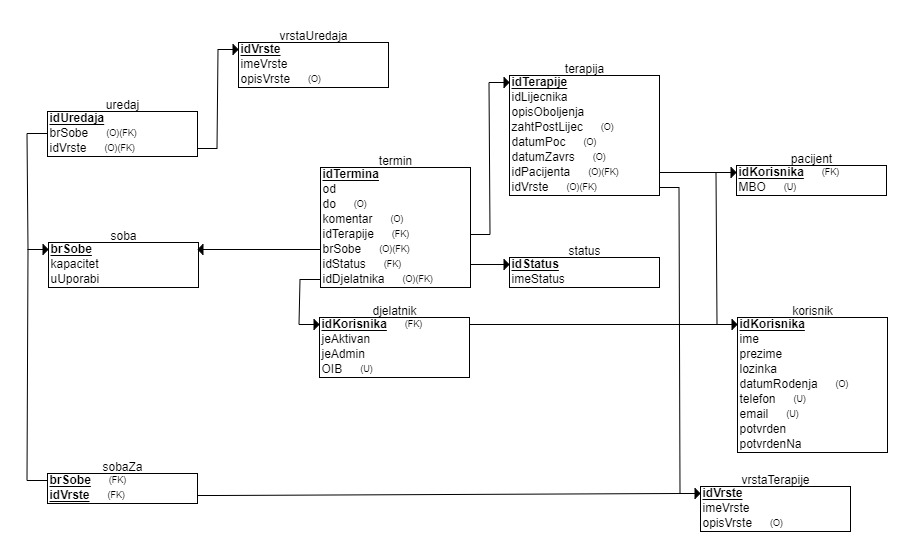
\includegraphics[width=\textwidth]{slike/Relacijska_shema_baze_podataka.JPG} %veličina u odnosu na širinu linije
			\caption{Relacijska shema baze podataka}
			\label{fig:relacijska_shema1} %label mora biti drugaciji za svaku sliku
		\end{figure}
		
		\begin{figure}[H]
			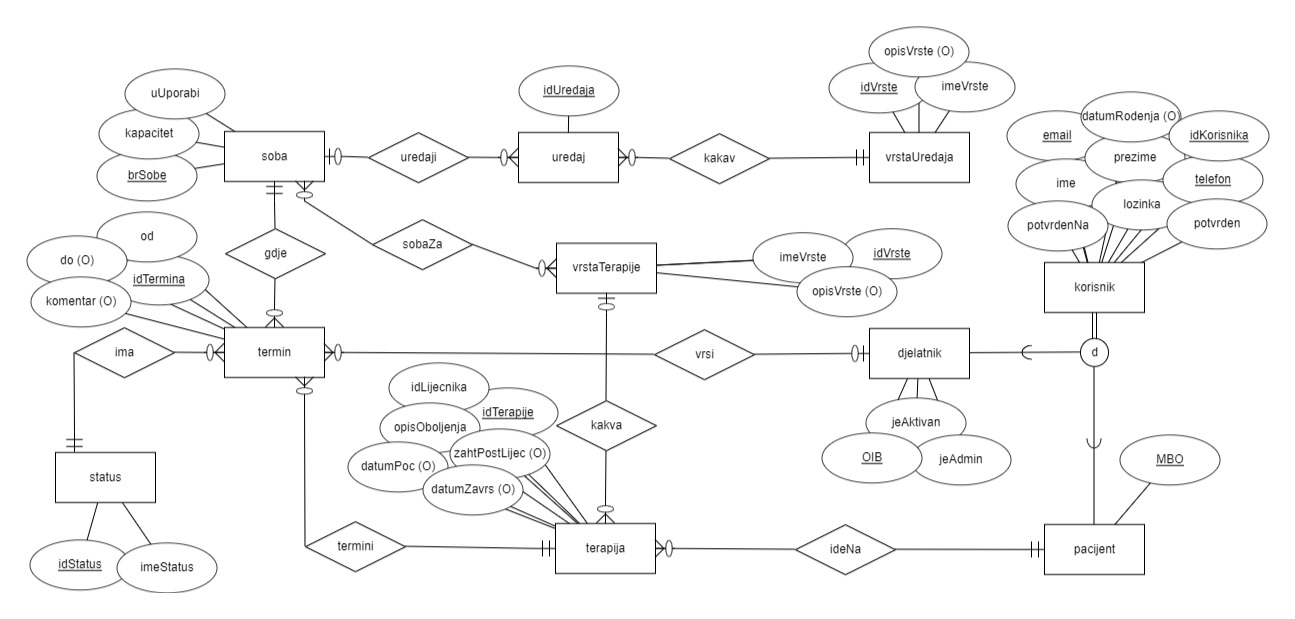
\includegraphics[width=\textwidth]{slike/ER_model_baze_podataka.JPG} %veličina u odnosu na širinu linije
			\caption{ER model baze podataka}
			\label{fig:er_model} %label mora biti drugaciji za svaku sliku
		\end{figure}
			
		\section{Dijagram razreda}
		
			Dijagrami razreda rađeni su po uzoru na MVC obrazac po kojem je naša aplikacija organizirana. Podijeljeni su u 3 dijela: Nadglednik(\textit{Controller}) (\ref{fig:dijagram_razreda_1}), DTO (\ref{fig:dijagram_razreda_2}) i Model (\ref{fig:dijagram_razreda_3}).
			
			Nadglednik obrađuje zahtjeve korisnika i preko DTO-a(\textit{Data transfer object}) vrši operacije nad Modelom. Zamišljeno je da funkcije implementirane u Nadgledniku vraćaju html status kod. \textit{KorisnikController} treba imati funkcije dobavljanja podataka i izmjene osobnih podataka. \textit{DjelatnikController} mora imati funkcije dobavljanja pacijenta i termina, evidencije pacijenta i dodavanje zahtjeva. \textit{PacijentController} mora imati funkcije dobavljanja zahtjeva, termina i nalaza, filtraciju termina i postavljanje terapije. \textit{AdminController} treba moći dobavljati djelatnike i termine, mijenjati djelatnike i termine, brisati djelatnike, sobe, uređaje i termine, dohvaćati djelatnike, sobe i uređaje i obavještavati pacijente. \textit{HomeController} treba imati pristup bazi i treba imati funkcije registracije i prijave.
			
			\begin{figure}[H]
				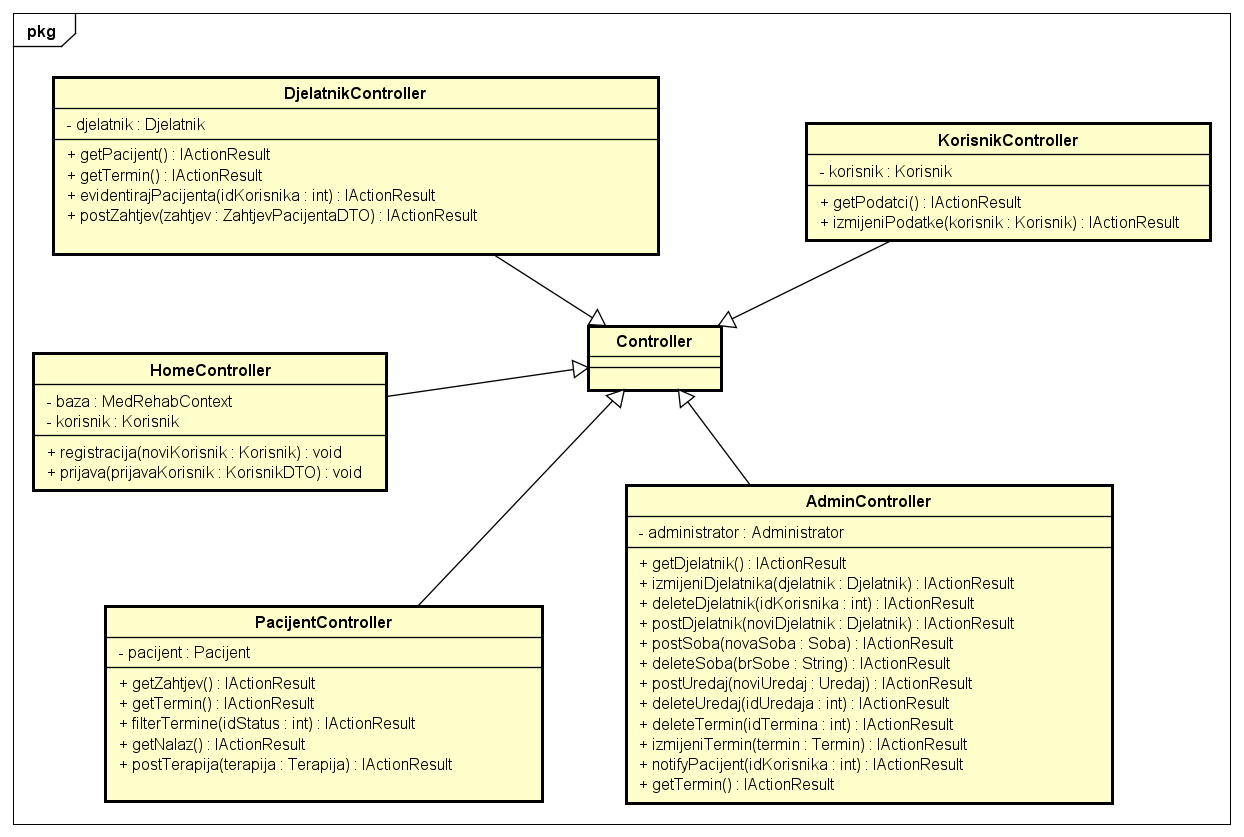
\includegraphics[scale=0.4]{slike/Dijagram_razreda_3.PNG} %veličina slike u odnosu na originalnu datoteku i pozicija slike
				\centering
				\caption{Dijagram razreda za dio Controller}
				\label{fig:dijagram_razreda_1}
			\end{figure}
			
			Dio s DTO-om sadrži jednostavne klase i služi isključivo za prenošenje podataka kako bi Nadglednik mogao vršiti operacije nad Modelom. Sadrži klase slične dijagramu razreda za dio Model uz nekoliko iznimaka. \textit{TerapijaSTerminima} sadrži atribute terapije s listom termina koji su vezanu uz pojedinu terapiju. \textit{ZahtjevPacijentaDTO} sadrži atribute Terapije i Termina koji su potrebni da bi Pacijent mogao napraviti Zahtjev.
			
			\begin{figure}[H]
				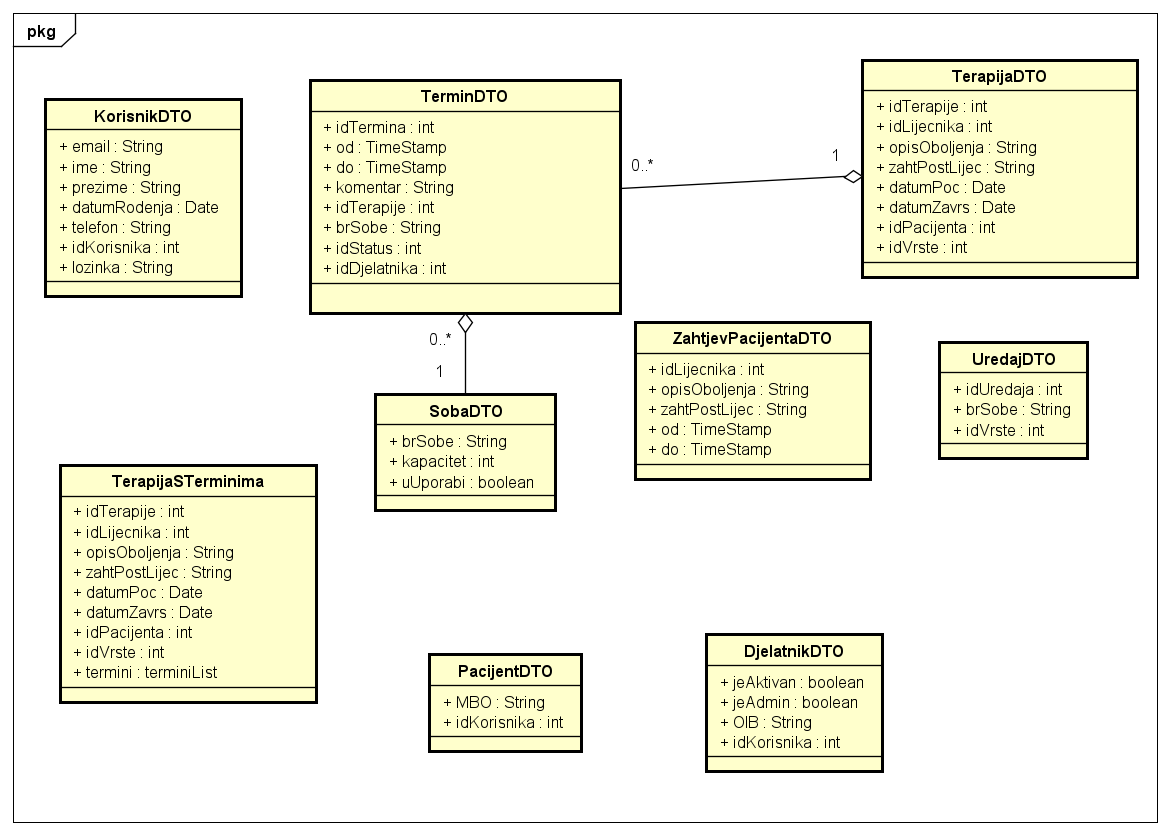
\includegraphics[scale=0.4]{slike/Dijagram_razreda_2.PNG} %veličina slike u odnosu na originalnu datoteku i pozicija slike
				\centering
				\caption{Dijagram razreda za dio DTO}
				\label{fig:dijagram_razreda_2}
			\end{figure}
			
			Model sadrži atribute i metode koje su potrebne radi komunikacije s bazom podataka. Razred \textit{Korisnik} predstavlja korisnika koji, ako je neprijavljen, ima funkciju registracije, a ako je prijavljen, ima funkciju prikaza i promjene osobnih podataka. \textit{Administrator} predstavlja korisnika koji upravlja djelatnicima, sobama i uređajima i obavještava pacijenta ukoliko je potrebno. \textit{Djelatnik} je liječnik koji ima opciju pregleda pacijenta, njegovih termina i evidencije njegovih termina, evidencije pacijenta i prihvaćanje ili odbijanje zahtjeva za terminom. Razred \textit{Pacijent} je pacijent koji može pregledati predane zahtjeve i termine, filtrirati termine, pregledati nalaze terapije i naručiti novu terapiju. Prisutne su i klase Terapija, vrstaTerapije, Termin, Status, Soba, Uredaj i VrstaUredaja koje za sada nemaju predviđene nikakve funkcije. Svaki razred sadrži atribute bitne za taj razred.
			
			\begin{figure}[H]
				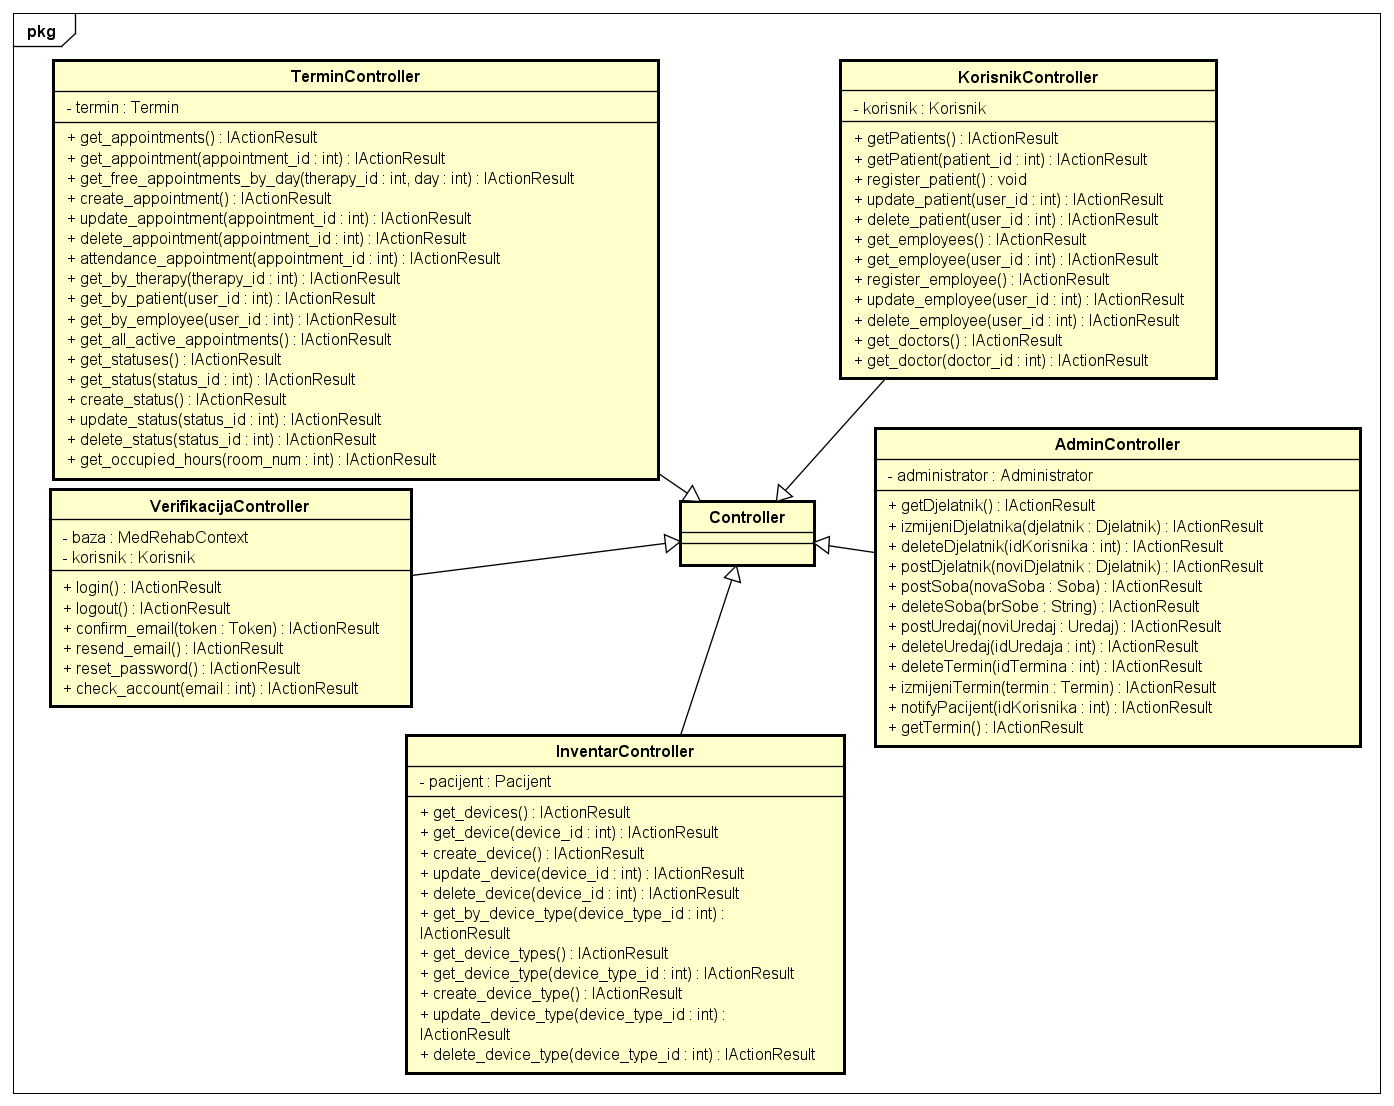
\includegraphics[scale=0.3]{slike/Dijagram_razreda_1.PNG} %veličina slike u odnosu na originalnu datoteku i pozicija slike
				\centering
				\caption{Dijagram razreda za dio Model}
				\label{fig:dijagram_razreda_3}
			\end{figure}
			
			
			
			\textbf{\textit{dio 2. revizije}}\\			
			
			\textit{Prilikom druge predaje projekta dijagram razreda i opisi moraju odgovarati stvarnom stanju implementacije}
			
			
			
			\eject
		
		\section{Dijagram stanja}
			
			
			\textbf{\textit{dio 2. revizije}}\\
			
			\textit{Potrebno je priložiti dijagram stanja i opisati ga. Dovoljan je jedan dijagram stanja koji prikazuje \textbf{značajan dio funkcionalnosti} sustava. Na primjer, stanja korisničkog sučelja i tijek korištenja neke ključne funkcionalnosti jesu značajan dio sustava, a registracija i prijava nisu. }
			
			
			\eject 
		
		\section{Dijagram aktivnosti}
			
			\textbf{\textit{dio 2. revizije}}\\
			
			 \textit{Potrebno je priložiti dijagram aktivnosti s pripadajućim opisom. Dijagram aktivnosti treba prikazivati značajan dio sustava.}
			
			\eject
		\section{Dijagram komponenti}
		
			\textbf{\textit{dio 2. revizije}}\\
		
			 \textit{Potrebno je priložiti dijagram komponenti s pripadajućim opisom. Dijagram komponenti treba prikazivati strukturu cijele aplikacije.}